\documentclass[11pt,a4paper]{article}

\usepackage[utf8]{inputenc}
\usepackage[T1]{fontenc}
\usepackage[margin=2.5cm]{geometry}
\usepackage{amsmath, amssymb}
\usepackage{booktabs}
\usepackage{graphicx}
\usepackage{siunitx}
\usepackage{xcolor}
\usepackage{hyperref}
\usepackage{eurosym}
\usepackage{titling}

\graphicspath{{figures/}}

\title{\textbf{Automatic Subreddit Classification of Reddit Posts}}
\author{Claudio Guarrasi\\[1ex]}
\date{\today}

% Subtitle above title (use \pretitle)
\pretitle{%
  \begin{center}
  	\vspace{-3cm} %vertical distance between upper margin and the logo. A negative value means that I am trying to get them closer.
  	\hspace*{0.1cm} %moving it on the right-
    	
\includegraphics[width=0.3\textwidth]{black_unipv_logo_caption_below.png}
	\rule{\textwidth}{0.3pt}
    	\textit{Machine Learning}\\[1ex]
    	\Large  % Switch to large font for the title
}
\posttitle{%
	\end{center} % Close centering.
	}

\preauthor{\begin{center}}
\postauthor{%
	\small{Department of Electrical, Computer and Biomedical Engineering}\\
	\small{University of Pavia}\\[1ex]
	\small{Email: \href{mailto:claudio.guarrasi01@universitadipavia.it}{claudio.guarrasi01@universitadipavia.it}}\\
	%\small{GitHub: \href{https://github.com/PapiDrago/n-body-problem}{\underline{https://github.com/PapiDrago/n-body-problem}}}
	\end{center}}



\begin{document}
\maketitle
\begin{abstract}
 We build classifiers that assign one of ten subreddits to a Reddit post from its title, body, comment count, and score. After an exploratory analysis showing that the numeric features encode post virality rather  than topic, and that the moderation tags [deleted]/[removed] constitute label leakage, we compare four models on a bag-of-words representation: multinomial naive Bayes (test accuracy 0.739), multinomial logistic regression (0.775), a linear SVM (0.779), and a multilayer perceptron (0.804). An ablation study answers the company's specific question: the number of comments and the score add roughly 1.8 accuracy points on historical data, but are near-constant on newly created posts and thus of little practical value at deployment. Error analysis shows a single failure --- news posts misclassified as business --- persisting identically across all four model families, identifying it as a property of the data: the news class lacks a distinctive vocabulary.
\end{abstract}

\tableofcontents





% ------------------------------------------------------------------
\section{Introduction}
\label{sec:intro}
This report addresses the classification of Reddit posts.
Reddit is an American social media platform inspired by internet forums from the early 2000s. In fact the Reddit platform is organized by user-created forum-like boards called "subreddits". Each subreddit typically focuses on a particular topic and follows moderation rules that may be different from the others.
Registered users submit content to the site such as links, text posts, images, and videos, which are then voted up or down ("upvoted" or "downvoted") by other members.
As of May 2026, Reddit is one of the most-visited websites in the world according to traffic data from the digital marketing platform Semrush~\cite{semrush2026}.

A company wants to implement a system that automatically places new content in the suitable subreddit. For a preliminary test, they selected ten subreddits: "Art", "Jokes", "Music", "anime", "business", "cats", "gaming", "movies", "news", "politics".

\section{Problem and data analysis}
\label{sec:eda}

\subsection{Problem}
The dataset consists of two \texttt{csv} files: a training set of 90{,}000
lines and a test set of 10{,}000 lines. Each line is a Reddit post with five
fields separated by the \texttt{|} character: \texttt{subreddit} (the label),
\texttt{num\_comments}, \texttt{score} (upvotes minus downvotes),
\texttt{title} (always present), and \texttt{text} (the body, which may be
empty or replaced by the tags \texttt{[deleted]} or \texttt{[removed]}).
For example, the line \texttt{Jokes|1|7|To be Frank,|[deleted]} is a post from
the \texttt{Jokes} subreddit with 1 comment, score 7, whose body was deleted.
We verified that every line contains exactly four separators, so parsing is
unambiguous. The goal is to build classifiers that assign a subreddit to a
brand-new post.

\subsection{Exploratory data analysis}
\label{subsec:eda}
Classes are perfectly balanced: 9000 training and 1000 test posts per
subreddit. All analyses below are on the training set.

\paragraph{Numeric features.}
Table~\ref{tab:numeric-describe} summarizes \texttt{num\_comments} and
\texttt{score}. Both are heavy-tailed: the medians are 1 comment and score 1,
while the means (16.1 and 180.8) are inflated by a small viral tail (maxima
above $9\times10^4$ and $10^5$). Crucially, the median post coincides with the
\emph{start default} of a brand new submitted post (0 comments, score 1
from the author's automatic upvote). These features therefore encode the
virality and longevity a post \emph{accumulates after} submission, not its
topic --- and since the company must classify a post at creation time, when
both features still sit at their defaults, they are near-constant exactly when
they would be needed. This does not imply they are useless for classification
in general; their contribution is quantified in
Section~\ref{sec:ablation}. Finally, although the score is defined as upvotes
minus downvotes, no post has a negative score: the data appear floored at
zero. A possible explanation is that the collection captured a display value
clipped at zero, though we cannot confirm the mechanism.

\paragraph{Body text.}
Table~\ref{tab:body-subreddit} breaks down the body field by status. Only
11{,}136 posts ($12\%$) carry usable body text; 51{,}451 are empty (typically
image or link posts) and 27{,}413 contain only the \texttt{[deleted]} or
\texttt{[removed]} tag. The title, always present, will therefore carry most
of the topic signal. The status distribution varies sharply by class:
\texttt{Jokes} is the only subreddit whose body is never empty (57\% present
--- likely a subreddit policy --- amounting to 46\% of \emph{all} text-bearing
posts, so body presence alone is a Jokes-leaning signal), image-centric
subreddits (\texttt{cats} 75\%, \texttt{business} 81\%, \texttt{news} 88\%
empty) put their content or link in the title, and \texttt{news} and
\texttt{politics} contain no removed posts at all. Body \emph{presence} is
thus itself informative, which motivates encoding it as an explicit feature
(Section~\ref{sec:extraction}).

\begin{table}[h]\centering\small
\caption{Summary statistics of the numeric features on the training set. The median post (1 comment, score 1) coincides with the cold-start default of a freshly submitted post, while the means are pulled up by a heavy viral tail (note the standard deviations and maxima).}
\label{tab:numeric-describe}
\begin{tabular}{lrr}\toprule & \texttt{num\_comments} & \texttt{score}\\\midrule
mean  & 16.14 & 180.79\\
std   & 346.28 & 2008.30\\
min   & 0 & 0\\25\%  & 0 & 1\\50\%  & 1 & 1\\75\%  & 3 & 7\\
max   & 91{,}283 & 103{,}279\\\bottomrule
\end{tabular}
\end{table}

\begin{table}[htbp]\centering\small
\label{tab:body-subreddit}
\caption{Body-text status per subreddit (fraction of training posts)}.\begin{tabular}{lcccc}\toprule
subreddit & deleted & empty & present & removed\\\midrule
Art & 0.32 & 0.60 & 0.01 & 0.07\\
Jokes & 0.16 & 0.00 & 0.57 & 0.27\\
Music & 0.26 & 0.54 & 0.06 & 0.14\\
anime & 0.20 & 0.27 & 0.30 & 0.22\\
business & 0.01 & 0.81 & 0.02 & 0.16\\
cats & 0.18 & 0.75 & 0.05 & 0.02\\
gaming & 0.20 & 0.58 & 0.14 & 0.08\\
movies & 0.16 & 0.51 & 0.09 & 0.24\\
news & 0.12 & 0.88 & 0.00 & 0.00\\
politics & 0.23 & 0.77 & 0.00 & 0.00\\\bottomrule
\end{tabular}
\end{table}
% [Tables tab:numeric-describe and tab:body-subreddit unchanged — keep yours,
%  with \caption before \label and no stray period.]

% ==================================================================
\section{Feature extraction}
\label{sec:extraction}

\paragraph{The status tags leak.}
The tags \texttt{[deleted]} (author removed the post) and \texttt{[removed]}
(moderators removed it) appear in 27{,}413 training posts, at rates that vary
strongly by class (e.g.\ 27\% of \texttt{Jokes} vs.\ 0\% of \texttt{news}).
Left in the vocabulary, they would be highly informative --- but the
information is spurious: both states arise only \emph{after} submission, are
produced by each subreddit's own moderation, and cannot exist on the
brand-new posts the company needs to classify. A model exploiting them would
partly learn ``removed-ness by subreddit'', a signal causally downstream of
the label and absent at inference time. We therefore strip both tags (and
URLs) from the text before building the vocabulary, and encode the body
status as a separate four-way categorical feature
(\texttt{present}/\texttt{empty}/\texttt{deleted}/\texttt{removed}). Following
the same reasoning as for the numeric features, the status feature is
excluded from the deployment model; both are retained for the controlled
comparison of Section~\ref{sec:ablation}, which quantifies exactly what they
contribute.

\subsection{Text representation}
Title and body are concatenated and represented as bag-of-words: each post
becomes a vector whose $i$-th entry counts the occurrences of vocabulary word
$i$. The vocabulary is learned from the training set only. We drop words
appearing in fewer than 10 posts --- accuracy was essentially unchanged
between thresholds 5 and 10, and fewer words means fewer parameters (the
logistic-regression weight matrix is $k \times n$ for $k$ classes and $n$
words) --- and apply Snowball stemming to merge inflectional variants such as
\texttt{cat}/\texttt{cats}. The final vocabulary has 8124 words
(\texttt{min\_df}=10, stemmed), down from 17{,}034 (\texttt{min\_df}=5,
unstemmed).

\subsection{Numeric features}
\texttt{num\_comments} and \texttt{score} are transformed by $\log(1+x)$
(plain $\log$ is undefined at the zeros the data contain) to compress the
heavy tail, then standardized to zero mean and unit variance. The
standardization parameters are estimated on the training set and applied
unchanged to the test set, so no test information enters the preprocessing;
the same fit-on-train discipline is applied to the vocabulary and all other
transformers.
% ------------------------------------------------------------------
\section{Models}
\label{sec:models}
We train four classifiers spanning three model families --- generative
(multinomial naive Bayes), discriminative linear (multinomial logistic
regression and a linear SVM), and non-linear (a multilayer perceptron) ---
all on the feature pipeline of Section~\ref{sec:extraction}. Unless stated
otherwise, models use the text counts plus the standardized numeric
features; every hyperparameter is selected by 5-fold cross-validation on
the training set only, and in each case the optimum lies in the interior
of the searched grid. The question this section answers is how far
bag-of-words features can go, and how much the choice of model family
matters on top of them.
\subsection{Multinomial logistic regression}
Logistic regression is discriminative: it models the posterior
$P(\text{class} \mid \mathbf{x})$ directly through one linear score per
class combined by a softmax, yielding piecewise-linear decision
boundaries. Standardizing the numeric features matters here because the
$L_2$ penalty shrinks all weights equally regardless of the scale of the
corresponding feature. Cross-validation over $C \in \{0.3, 1, 3, 10\}$ selects $C = 1$. The model reaches a test accuracy of 0.775 with a train accuracy of 0.859; attempts to close this gap by pruning the vocabulary reduced overfitting but never improved test accuracy (Figure~\ref{fig:mindf}), indicating that the ceiling is set by the bag-of-words representation rather than by under or
over regularization.
\begin{figure}[htbp]
    \centering
    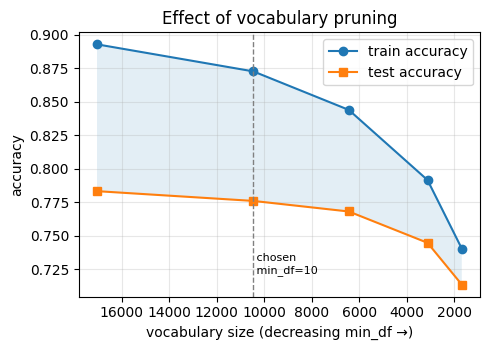
\includegraphics[width=0.6\linewidth]{mindf_sweep.png}
    \caption{The test\//training accuracy gap shrinks as we prune.}
    \label{fig:mindf}
\end{figure}
\subsection{Multinomial naive Bayes}
Naive Bayes is the generative counterpart: it models the class-conditional
distribution $P(\text{words} \mid \text{class})$ under the assumption that
words are conditionally independent given the class, so the joint
likelihood factorizes into a product of per-word probabilities. At
inference time the prediction is the argmax over classes of the log-prior
plus the sum of per-word log-likelihoods. Because it treats
a document as a realization of a multinomial over word counts, it cannot
accommodate the standardized (negative-valued) numeric features and is
trained on text counts only. The smoothing parameter is set to
$\alpha = 0.3$ by cross-validation. We obtained a training accuracy of 0.757 and a test accuracy 0.739, with a gap of only 0.02: the independence assumption prevents the model from representing word correlations, so it underfits even the training set, but for the same reason it barely overfits. Its $\sim$2-point deficit to logistic
regression is the measured cost of that assumption.
 
\subsection{Linear SVM}
The linear SVM replaces the cross-entropy loss with the hinge loss and
seeks the separating hyperplane of maximum margin.
Multiclass classification uses the one-vs-rest scheme: ten hyperplanes,
one per class, with the prediction given by the largest signed margin
$\mathbf{w} \cdot \mathbf{x} + b$ (proportional to the distance from each
hyperplane). Cross-validation selects $C = 0.1$ --- stronger regularization than logistic regression, as is typical for the hinge loss on sparse text. With
test accuracy 0.779 it is the strongest linear model, and it also overfits
slightly less than logistic regression (train 0.847).
 
\subsection{Multilayer perceptron}
The MLP is the only non-linear model: a single hidden layer of 256 ReLU
units with dropout 0.5, mapping the 8126 input features to the 10 class
logits, trained in PyTorch on GPU with Adam and weight decay $10^{-4}$
(batches are densified row-by-row from the sparse matrix). Training and testing exhibit the expected divergence i.e.\ the MLP model overfits, which we control by early stopping on a 10\% validation split carved from the training set
(patience 3, restoring the best-validation weights). The early-stopped
model reaches a test accuracy of 0.804: the hidden layer captures word
co-occurrence patterns that no linear model on independent word features
can represent.
 
\begin{table}[htbp]\centering\small
\caption{Final test performance. All models use text + numeric features
except naive Bayes (text only, see above).}
\label{tab:results}
\begin{tabular}{lccc}\toprule
Model & train acc. & test acc. & macro-F1\\\midrule
Multinomial NB ($\alpha=0.3$) & 0.757 & 0.739 & 0.735\\
Logistic regression ($C=1$)   & 0.859 & 0.775 & 0.776\\
Linear SVM ($C=0.1$)          & 0.847 & 0.779 & 0.778\\
MLP (early-stopped)           & 0.861 & 0.804 & 0.804\\
\bottomrule
\end{tabular}
\end{table}
 
Table~\ref{tab:results} summarizes the comparison. Two patterns stand out.
First, the three linear models cluster within four points of one another
(0.739--0.779), with the ordering NB $<$ LR $<$ SVM reflecting thar the more assumptions a model relaxes, the more signal it extracts, at the price of a larger train/test gap. Second, the single non-linear model gains a further 2.5 points over the best linear one --- evidence that word \emph{interactions} carry real signal beyond individual word occurrences. Since macro-F1 tracks accuracy closely for
every model, no classifier is trading one class off against the others.
Which classes drive these differences, and why the remaining errors
persist across all four models, is the subject of Section~\ref{sec:behavior}.
% ------------------------------------------------------------------
\section{Special request: are the number of comments and the score useful?}
\label{sec:ablation}
The company specifically asked whether \texttt{num\_comments} and
\texttt{score} help in determining the subreddit. We answer it with an
ablation study: starting from a text-only model, we add the numeric features
and the status feature (Section~\ref{sec:extraction}) in turn and measure the
change in test accuracy. Table~\ref{tab:ablation} reports the result for
logistic regression; the same pattern was observed for the linear SVM, so the
conclusions are not specific to one model.
 
\begin{table}[htbp]\centering\small
\caption{Feature ablation (logistic regression, $C=1$, stemmed vocabulary).}
\label{tab:ablation}
\begin{tabular}{lccc}\toprule
Features & train acc. & test acc. & macro-F1\\\midrule
text only               & 0.846 & 0.758 & 0.758\\
text + numeric          & 0.859 & 0.775 & 0.776\\
text + status           & 0.864 & 0.776 & 0.776\\
text + numeric + status & 0.877 & 0.791 & 0.791\\\bottomrule
\end{tabular}
\end{table}
 
\paragraph{The direct answer.}
Empirically, yes: adding the numeric features raises test accuracy by about
1.8 points (0.758 to 0.775). The gain is real and, notably, additive with the
status feature (each contributes $\sim$1.8 points and together
$\sim$3.3), which means the two carry independent signal --- the
numeric features are not merely a proxy for post format. The likely source is
differential engagement: high-traffic subreddits such as \texttt{news} and
\texttt{politics} accumulate more comments and score than image-centric ones.
 
\paragraph{Why the gain is deployment-fragile.}
This 1.8-point improvement is measured on \emph{historical} posts, where
comments and score have accumulated over the post's lifetime. As established
in Section~\ref{subsec:eda}, a brand-new post --- the object the company
actually needs to classify --- sits at the cold-start default (0 comments,
score 1), which is precisely the dataset median. At that moment the two
features are near-constant across all subreddits and therefore carry almost no
discriminative information. The historical gain would largely evaporate at the
point of use. Our recommendation is thus qualified: the numeric features are
weakly informative in principle, but of little practical value for the
company's stated goal of classifying content at submission time.
 
\paragraph{Status quantifies a leak.}
The status feature adds a further $\sim$1.8 points, but this figure should be
read as a caution rather than an endorsement. As argued in
Section~\ref{sec:extraction}, the \texttt{[deleted]}/\texttt{[removed]} states
are produced \emph{after} submission by each subreddit's own moderation, so
the feature is causally downstream of the label and cannot exist on a new
post. The accuracy it contributes is therefore leaked: the
\texttt{text+numeric+status} figure of 0.791 is an upper bound inflated by a
signal unavailable at deployment, not a realistic estimate of field
performance. We exclude both status and the numeric features from the
deployment model, whose honest estimate is the text-based 0.76--0.80 of
Table~\ref{tab:results}; the numeric and status columns above serve only to
answer the company's question and to make the leakage explicit.

\section{Model behavior analysis}
\label{sec:behavior}
 
\subsection{Where the models fail and where they agree}
Table~\ref{tab:recall} reports the per-class recall (the diagonal of the
row-normalized confusion matrix) for all four models, and
Figure~\ref{fig:mlpcm} shows the full confusion matrix of the best model.
 
\begin{table}[htbp]\centering\small
\caption{Per-class recall by model. Bold marks each model's weakest class.}
\label{tab:recall}
\begin{tabular}{lcccc}\toprule
Class & NB & LR & SVM & MLP\\\midrule
Art      & 0.80 & 0.80 & 0.81 & 0.85\\
Jokes    & 0.71 & 0.75 & 0.76 & 0.77\\
Music    & 0.82 & 0.82 & 0.83 & 0.82\\
anime    & 0.76 & 0.79 & 0.80 & 0.80\\
business & 0.75 & 0.82 & 0.81 & 0.81\\
cats     & 0.79 & 0.89 & 0.90 & 0.90\\
gaming   & 0.65 & 0.71 & 0.70 & 0.73\\
movies   & 0.73 & 0.75 & 0.76 & 0.76\\
news     & \textbf{0.50} & \textbf{0.58} & \textbf{0.54} & \textbf{0.62}\\
politics & 0.86 & 0.86 & 0.89 & 0.91\\\bottomrule
\end{tabular}
\end{table}
 
Two regularities cut across all four models. First, the easiest classes are
those with a distinctive, dedicated vocabulary: \texttt{cats} and
\texttt{politics} exceed 0.86 recall in every discriminative model. Second,
and more strikingly, \texttt{news} is the weakest class in \emph{all four}
models, and in all four it is confused primarily with \texttt{business}, at an
almost identical rate (0.21 for NB, 0.22 for LR, 0.24 for SVM, 0.23 for the
MLP). Four model families --- generative, two discriminative-linear, and
non-linear --- fail on the same class, in the same direction, by the same
amount. This convergence shows the failure is a property of the
\emph{dataset}, not of any algorithm.
 
The comparison across models is equally informative. Naive Bayes suffers most
on \texttt{gaming} (0.65), a ``multidisciplinary'' topic whose signal lies in
word \emph{combinations} that the independence assumption cannot represent;
on classes with strong marker words (\texttt{Music}, \texttt{politics}) it
matches logistic regression exactly, since there independence costs nothing.
The SVM improves precisely the classes that are already well separated ---
margin maximization sharpens boundaries where a boundary exists --- while on
\texttt{news}, which has no clean margin to exploit, it does slightly worse
than logistic regression. The MLP lifts nearly every class and recovers
\texttt{gaming} to 0.73, directly exhibiting the value of learned word
interactions; yet even the MLP leaves the news$\to$business confusion intact.
Interactions can be learned where they exist; they cannot be manufactured
where the vocabularies genuinely overlap, as when a news post about the
economy is written in the language of \texttt{business}.
 
\subsection{High-confidence errors}
Ranking misclassifications by the model's confidence (predicted-class
probability for logistic regression; the margin gap between predicted and
true class for the SVM, which yields a consistent picture) reveals two
failure mechanisms. The first is \emph{misleading signal}: posts whose words
genuinely point to another class, either because the content is legitimately
cross-topic (``Gaming equivalents to movies that made you think'', a
\texttt{gaming} post saturated with movie vocabulary; a \texttt{news} post on
an NRA investigation predicted as \texttt{politics}, where the true label is
itself arguable) or because of a homonym collision (posts about the film
\emph{Cats} classified as \texttt{cats}). The second is \emph{absent signal}:
titles with no topical words at all (``Air Fresheners'', ``stone pc''), where
the model has nothing to condition on and even a human would struggle.
 
Notably, the most \emph{confident} errors and the most \emph{frequent} error
are disjoint: no news$\to$business mistake appears among the top-confidence
misclassifications. The dominant error is made hesitantly --- many news posts
drift to business, but never with conviction --- exactly as expected for a
class with no strong vocabulary of its own. Frequency and confidence thus
rank different failure modes: the former exposes the data's structural
overlap, the latter the representation's blind spots. Both are properties of
the task and the bag-of-words representation rather than deficiencies any of
the tested models could overcome.
 
% Figures: keep the MLP confusion matrix + the two-panel diagnostics here.
\begin{figure}[htbp]\centering
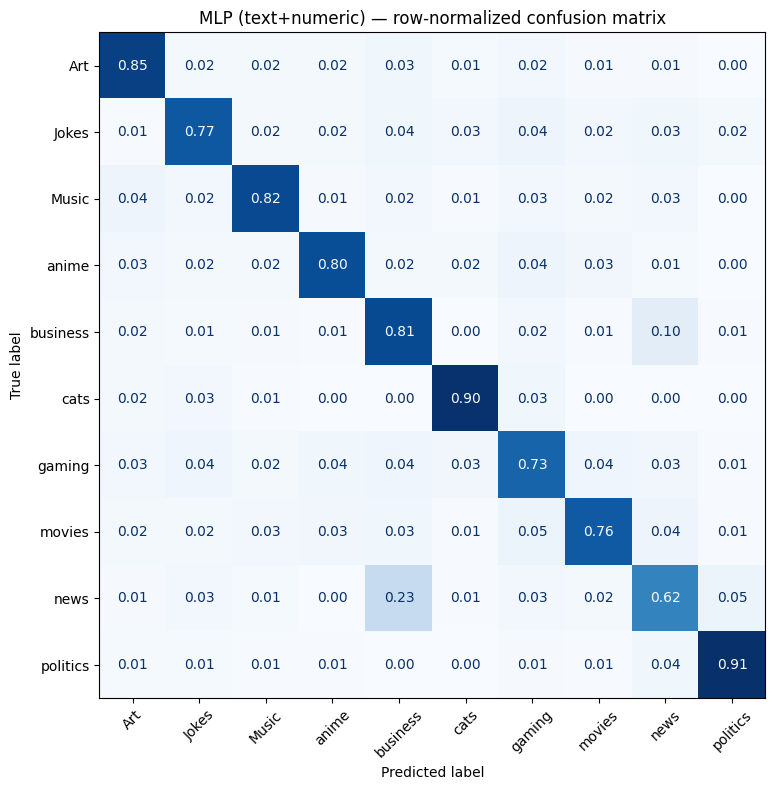
\includegraphics[width=.7\linewidth]{mlp_conf_matrix.png}
\caption{Row-normalized confusion matrix of the MLP (best model). The
news$\to$business cell (0.23) persists at the same magnitude as in all three
linear models.}
\label{fig:mlpcm}
\end{figure}
 
% ------------------------------------------------------------------
\section{Conclusions}
\label{sec:conclusions}
Text does the work: bag-of-words over title and body takes a 10-class problem
from 0.10 chance accuracy to 0.74--0.78 with linear models, and to 0.80 with
an MLP whose hidden layer captures word co-occurrence. The remaining ceiling
is set by the representation --- word counts with no order or semantics ---
rather than by model capacity, as shown by the failure of both regularization
and vocabulary pruning to improve test accuracy. On the company's specific
question: the number of comments and the score add a small ($\sim$1.8-point),
model-independent gain on historical data, but both features sit at a
near-constant cold-start default on the brand-new posts the system must
classify, so we recommend the deployed classifier rely on text alone. The
post-status feature is excluded as leaky. Finally, the news$\to$business
confusion persists identically across all four model families: separating
these two classes would require richer features than word counts, or should
simply be accepted as genuine topical overlap.
 
% ------------------------------------------------------------------
\section*{Declaration of AI-tool usage}
AI assistance (Anthropic's Claude) was used for the following tasks:
planning the analysis pipeline and the ablation design; drafting and
debugging Python code (data-integrity checks, vectorization, model training
and evaluation, diagnostic plots; identifying the \texttt{LinearSVC}
dual-solver convergence issue); discussing the interpretation of results
(the leakage of the status feature, the reading of confusion matrices and
of the ablation study); reviewing and correcting the author's written
comments; and drafting the structure and parts of the text of this report,
subsequently revised by the author. All experiments were executed, and all
results verified, by the author.
% TODO: adjust so it reflects exactly what you used AI for — accuracy of
% this declaration is your responsibility.
 
\bigskip
\noindent\textit{I affirm that this report is the result of my own work and
that I did not share any part of it with anyone else except the teacher.}


\begin{thebibliography}{9}
 
\bibitem{semrush2026}
\newblock \url{https://www.semrush.com/trending-websites/global/all}.
\newblock Accessed on 06/07/26.
 
\end{thebibliography}


\end{document}
